\documentclass[../main.tex]{subfiles}

\begin{document}
\chapter{Konstruktion der Reellen Zahlen}
\section{Historische Motivation}
In der Antike war Mathematik praktisch synonym mit Geometrie. Der Zahlenbegriff war
direkt an das Konzept der \textit{Länge} gekoppelt.

\begin{definition}[Euklid, 300 vor Christus]
  Zwei Längen $a,b > 0$ heissen \textit{kommensurabel}, falls eine Länge $L>0$ existiert,
  so wie zwei natürliche Zahlen $m,n \in \mathbb N$, so dass $a = mL$ und $b=nL$.
\end{definition}

Hier ist
\[\mathbb N = \{0, 1, 2, 3, 4, \dots\}\]
die Menge der Natürlichen Zahlen.

\begin{theorem}[Euklid]
  Die Seite und Diagonale eines ebenen Quadrats sind nicht kommensurabel.
\end{theorem}

\begin{proof}
  Dieser Beweis ist geometrisch, nach Euklid. Wir nehmen an, es gäbe $L > 0$ und
  $m,n \in \mathbb N$ mit $x = mL$ und $d = nL$. Wir zeigen, dass das zu einem Widerspruch
  führt.
  Wir stellen fest, dass die Längen $x_{1} = d-x$ und $d_{1} = 2x - d$
  ebenfalls die Seite und Diagonale eines Quadrats bilden, siehe
  Abbildung~\ref{fig:euklid}.

  \begin{figure}[htb]
    \centering
    \begin{minipage}{0.4\linewidth}
      \centering
      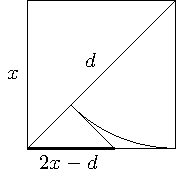
\includegraphics{images/euklid-quadrat}
    \end{minipage}%
    \begin{minipage}{0.4\linewidth}
      \centering
      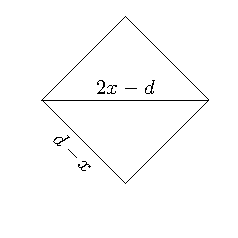
\includegraphics{images/euklid-quadrat2}
    \end{minipage}
    \caption{Euklids Konstruktoin}%
    \label{fig:euklid}
  \end{figure}

  Weiterhin gilt, dass sowohl $x_{1}$ als auch $d_{1}$, ganze Vielfache von $L$ sind:
  \begin{align*}
    x_{1} = d-x = (n-m)L \\
    d_{1} = 2x-d = (2m -n)L
  \end{align*}
  Nach Pythagoras gilt $d^{2} = 2x^{2}$, und somit $d \leq 3/2\cdot x$, da ${(3/2)}^{2} > 2$.
  Daraus folgt, dass
  \[x_{1} = d - x \leq \frac{1}{2} \cdot x.\]
  Iteriere dieses Verfahren und erhalte eine Serie von Quadraten mit Seiten
  $x_{2}, x_{3}, \dots$ und Diagonalen $d_{2}, d_{3}, \dots$. Es gilt:
  \[x_{k} \leq \frac{1}{2^{k}} \cdot x.\]
  Ausserdem ist jedes $x_{k}$ (und $d_{k}$) ein ganzes Vielfaches von $L$.
  Wähle nun $k$ so gross, dass
   \[x_{k} \leq \frac{1}{2^{k}} x < L.\]
   Dies impliziert, dass $x_{k} = 0$, was unmöglich ist. Deshalb können $x$ und $d$
   nicht kommensurabel sein.
\end{proof}

Wir haben diese Aussage mit einem sogenannten \textit{Widerspruchsbeweis} bewiesen.
Hierfür haben wir eine Annahme getroffen, und diese zu einem Widerspruch geführt.
Dies zeigt, dass unsere Annahme falsch war.

\subsection*{Zeitgenössische Umformulierung}
Seien $a,b > 0$ zwei kommensurable Längen. Das heisst, es existieren $L > 0$
und $m,n \in \mathbb N$ mit $a = mL$, $b= nL$. Dann gilt:
\[\frac{a}{b} = \frac{mL}{nL} = \frac{m}{n},\]
das heisst das Verhältnis $a/b$ ist eine \textit{rationale Zahl}.
Zurück zum Quadrat mit Seite $x$ und Diagonale $d$. Nach Pythagoras
gilt $d^{2} = 2x^{2}$. Falls $x=mL$ und $d=nL$ gilt,
dann also
\[2 = \frac{d^{2}}{x^{2}} = {\left( \frac{d}{x}\right)}^{2} = {\left(\frac{n}{m}\right)}^{2},\]
und somit
\[2m^{2} = n^{2}.\]
Die linke Seite dieser Gleichung ist durch $2$ teilbar. Dies impliziert, dass $n^{2}$, und
somit auch $n$, durch $2$ teilbar ist. Schreibe nun $n = 2k$. Schreibe $n = 2k$ mit
$k \in \mathbb N$. Setze ein und erhalte
$2m^{2} = {(2k)}^{2} = 4k^{2}$,
beziehungsweise
\[m^{2} = 2k^{2}.\]
Die rechte Seite ist durch $2$ teilbar, also auch $m$.
Wir schliessen, dass sowohl $n$ als auch $m$ durch $2$ teilbar sind.
Schreibe noch $m = 2\ell$ mit $\ell \in \mathbb N$. Es gilt also
\[ 2 = {\left(\frac{n}{m}\right)}^{2}
  = {\left(\frac{k}{\ell}\right)}^{2}.\]
In anderen Worten sind Zähler und Nenner beide gerade.
Iteriere dieses Verfahren $k$ mal, bis $n/2^{k} < 1$, Dann entsteht ein Widerspruch.

\begin{corollary}
  Die Gleichung $z^{2} = 2$ hat keine rationale Lösung, das heisst,
  keine Lösung der Form $z = p/q$ mit $p, q \in \mathbb N$ und $q > 0$.
\end{corollary}

Das Ziel für den Rest dieses Kapitels ist es, eine Zahlenmenge $\mathbb R$ (die Menge
der \textit{reellen Zahlen}) zu konstruieren, in welcher die Gleichung
$z^{2} = 2$ eine Lösung hat.

\begin{exercise}
  Die Gleichung $z = \sqrt 2 x + \sqrt 3 y$ hat keine ganze Lösungen ausser $(0,0,0)$.
\end{exercise}

\section{Mengen im Vergleich}
Wir haben bereits einige Mengen erwähnt, nämlich die \textit{natürlichen Zahlen}
\[ \mathbb N = \{0, 1, 2, 3, \dots\},\]
die Menge der \textit{ganzen Zahlen},
\[ \mathbb Z = \{0, 1, -1, 2, -2, \dots\},\]
und die Menge der \textit{rationalen Zahlen}
\[ \mathbb Q = \left\{p/q \mid p, q \in \mathbb Z, \, q > 0\right\}.\]
Wir wollen eine weitere Menge, die Menge $\mathbb R$ der \textit{reellen Zahlen}
einführen. Es gelten dann die Inklusionen
\[\mathbb N \subset \mathbb Z \subset \mathbb Q \subset \mathbb R.\]

\subsection*{Wichtige Grundbegriffe}
\begin{definition}
  Seien $A, B$ zwei Mengen. Eine Abbildung $f: A \to B$ heisst
  % TODO small roman
  \begin{enumerate}[(i)]
    \item \textit{injektiv}, falls für alle $a_{2}, a_{1} \in A$
      mit $a_{2} \ne a_{1}$ gilt, dass $f(a_{1}) \neq f(a_{2})$,
    \item \textit{surjektiv}, falls für alle $b \in B$ ein Element
      $a \in A$ existiert mit $f(a) = b$,
      \item \textit{bijektiv}, falls $f$ sowohl injektiv als auch surjektiv ist.
  \end{enumerate}
\end{definition}

\begin{example}\label{ex:inj-surj}
  \leavevmode
  \begin{enumerate}[(i)]
    \item Seien $A = B = \{0, 1\}$. Es gibt $4$ Abbildungen $f: A \rightarrow B$:
      \begin{enumerate}[(a)]
        \item $0 \mapsto 0$ und $1 \mapsto 0$,
        \item $0 \mapsto 1$ und $1 \mapsto 1$,
        \item $0 \mapsto 0$ und $1 \mapsto 1$,
        \item $0 \mapsto 1$ und $1 \mapsto 0$.
      \end{enumerate}
      Abbildungen (a) und (b) sind weder injektiv noch surjektiv. Abbildungen (c) und (d) sind
      beide bijektiv.
    \item Seien $A = B = \mathbb N$. Betrachte die Abbildung
      \begin{align*}
        f: & \;\mathbb N \rightarrow \mathbb N \\
        & \;n \mapsto 2n.
      \end{align*}
      Diese Abbildung ist injektiv, aber nicht surjektiv. Die Abbildung
      \begin{align*}
        g: & \;\mathbb N \rightarrow \mathbb N \\
           & \; n \mapsto \frac{2n - 1 + {(-1)}^{n}}{4},
      \end{align*}
      also die Abbildung die durch $2$ dividiert und dann abrundet, ist nicht injektiv,
      aber surjektiv. Um zu sehen, dass
      $g(n) = \lfloor{n/2}\rfloor$, betrachte zwei Fälle:
      \begin{enumerate}[(a)]
        \item $n = 2k$ ist gerade. Dann ist $g(n) = (4k+1-1)/4 = k$.
        \item $n = 2k + 1$ ist ungerade. Dann ist $g(n) = (4k + 2 -1 -1)/4 = k$.
      \end{enumerate}
  \end{enumerate}
\end{example}

\begin{remark}
  \leavevmode
  \begin{enumerate}[(1)]
    \item Bijektive Abbildungen $f: A \to B$ haben eine eindeutige \textit{Umkehrabbildung}
      $f^{-1}: B \to A$. Die Konstruktion dafür ist wie folgt. Sei $b \in B$.
      Da $f$ surjektiv ist, existiert $a \in A$ mit $f(a) = b$. Da $f$
      injektiv ist, ist dieses $a$ eindeutig. Setze $f^{-1}(b) = a$. Es gilt dann
      \[f^{-1}(f(a)) = a\]
      für alle $a \in A$, und ebenso
      \[f(f^{-1}(b))\]
      für alle $b \in B$. Wir schreiben häufig
      \begin{align*}
        f^{-1} \circ f = \textrm{Id}_{A}, \\
        f \circ f^{-1} = \textrm{Id}_{B},
      \end{align*}
      in Worten, ``$f^{-1}$ verknüpft mit $f$ ist die Identitätsabbildung auf $A$''
      und ähnlich, ``$f$ verknüpft mit $f^{-1}$ ist die Identitätsabbildung auf $B$''
    \item Für endliche Mengen $A$ und $B$ gilt: Es existiert eine bijektive Abbildung
      $f: A \to B$, genau dann, wenn $A$ und $B$ gleich viele Elemente haben.
  \end{enumerate}
\end{remark}

\begin{definition}
  Eine Menge $A$ heisst
  \begin{enumerate}[(i)]
    \item \textit{unendlich}, falls eine injektive, nicht surjektive Abbildung
      $f: A \to A$ existiert,
    \item \textit{abzählbar}, falls eine bijektive Abbildung $f: \mathbb N \to A$
      existiert.
  \end{enumerate}
\end{definition}

\begin{example}
  Sei $A = \mathbb N$. Die Abbildung $f$ aus Beispiel~\ref{ex:inj-surj} (ii) ist injektiv,
  aber nicht surjektiv. Also ist $\mathbb N$ eine unendliche Menge.
\end{example}

\begin{example}
  Sei $M$ eine Menge, welche $\mathbb N$ als Teilmenge enthält
  (zum Beispiel $M = \mathbb Q$).
  Dann ist $M$ unendlich. Betrachte dazu die Abbildung
  \begin{align*}
    f:\;& M \to M \\
    & x \mapsto
      \begin{cases}
        x+1 & \mbox{falls }x \in \mathbb N \subset M, \\
        x & \mbox{falls }x \in M \setminus \mathbb N
      \end{cases}
  \end{align*}
\end{example}

Folgende Proposition zeigt in einem gewissen Sinn, dass es gleich viele Brüche
wie natürliche Zahlen gibt. Dies ist unser erstes potentiell überraschendes
Resultat.

% TODO make this numbered
\begin{manualproposition}{1}
  Die Menge $\mathbb Q$ der rationalen Zahlen ist abzählbar.
\end{manualproposition}


\begin{proof}
  Wir konstruieren eine Bijektion $\varphi: \mathbb N \to \mathbb Q$.
  Für $k \in \mathbb N$ mit $k \geq 1$ definiere
  \[
    A_{k} = \left\{p/q \mid p, q \in \mathbb Z, q \geq 1, p/q \textup{ ist gekürzt},
    |p| + |q| = k\right\}.
  \]
  Alle solchen $A_{k} \subset \mathbb Q$ sind endlich und
  \[
    \mathbb Q = \bigcupdot_{k \geq 1} A_{k}
  \]
  ist die \textit{disjunkte Vereinigung} dieser Mengen.
  Wir haben
  \[
    A_{1} = \{0/1\}, \; A_{2} = \{\pm 1/1\}, \; A_{3} = \{\pm 1/2, \pm 2/1\}, \dots.
  \]
  Sei $a_{k} = |A_{k}|$ die Anzahl Elemente von $A_{k}$.
  Definiere Teilmengen $B_{k} \subset \mathbb N$ mit $|B_{k}| = a_{k}$.
  Dazu setze $B_{1} = \{0\}$, und für $k \geq 2$ setze
  \[
    B_{k} = \{a_{1} + \cdots + a_{k-1},
    a_{1} + \cdots + a_{k-1} + 1, \dots,
    a_{1} + \cdots + a_{k-1} + a_{k} - 1\}.
  \]
  Es gilt dann
  \[
    B_{1} = \{0\}, \; B_{2} = \{1, 2\}, \; B_{3} = \{3, 4, 5, 6\}, \dots.
  \]
Wähle eine Bijektion $\varphi_{k}: B_{k} \to A_{k}$ für alle $k \geq 1$.
Definiere nun
\begin{align*}
  \varphi: \;& \mathbb N \to \mathbb Q \\
  &n \mapsto \varphi_{k}(n) \mbox{ falls } n \in B_{k}.
\end{align*}
Die Abbildung $\varphi$ ist eine Bijektion, da $\mathbb N$ die disjunkte
Vereinigung der $B_{k}$ und $\mathbb Q$ die disjunkte Vereinigung
der $A_{k}$ ist.
\end{proof}

Dieser Beweis zeigt allgemeiner, dass jede Menge, die eine abzählbare Vereinigung
endlicher Mengen ist, selber abzählbar ist. Man könnte diese Aussage
für Aufgabe 5 auf Serie 1 verwenden.

\begin{question}
  Ist jede unendliche Menge abzählbar?
\end{question}

Georg Cantor hat ca. 1870 als erste Person die Antwort ``nein'' auf diese Frage
festgehalten. Dies wurde allerdings erst nach dem Krieg publiziert.
Wir konstruieren nun eine Menge, die nicht abzählbar ist.
Dazu betrachten wir die \textit{Potenzmenge} $P(M)$
einer Menge $M$, definiert als die ``Menge aller Teilmengen von $M$''.
Ein wenig formaler,
\[P(M) = \left\{A \mid A \subset M\right\}.\]

\begin{example}
  Sei $M = \{0, 1\}$. Dann ist
  \[
    P(M) = \{ \emptyset, \{0\}, \{1\} \{0, 1\}\}.
  \]
  Hier bedeutet $\emptyset$ die \textit{leere Menge}.
\end{example}

\begin{remark}
  Falls die Menge $M$ selbst $n$ Elemente hat, dann hat ihre
  Potenzmenge $2^{n}$ Elemente. Hierzu fassen wir jede Teilmenge $A$ von $M$
  als Funktion
  \begin{align*}
    f_{A}: \;& M \to \{0, 1\} \\
    & x \mapsto
      \begin{cases}
        0, & \mbox{falls } x \notin A, \\
        1, & \mbox{falls } x \in A,
      \end{cases}
  \end{align*}
  auf.
  Diese Funktion enthält die selbe Information wie $A$ selbst.
\end{remark}



% TODO number this
\begin{manualproposition}{2}[Cantor]
  Sei $M$ eine beliebige Menge.
  Dann existiert keine surjektive Abbildung $\varphi: M \to P(M)$.
  Insbesondere existiert keine Bijektion $\varphi: M \to P(M)$.
\end{manualproposition}

\begin{corollary}
  Die Potenzmenge $P(\mathbb N)$ ist nicht abzählbar.
\end{corollary}

\begin{proof}[Beweis der Proposition]
  Wir führen einen klassischen Widerspruchsbeweis.
  Wir nehmen an, es gäbe doch eine solche Surjektion
  $\varphi: M \to P(M)$.
  Betrachte nun die Teilmenge $A$ von $M$ aller $x$, die nicht
  in $\varphi(x)$ enthalten sind. In Symbolen,
  \[
    A = \left\{x \in M \mid x \notin \varphi(x)\right\}
  \]
  Die Forderung $x \notin \varphi(x)$ macht Sinn,
  da $\varphi(x)$ selbst eine Teilmenge von $M$ ist.
  Da $\varphi$ surjektiv ist, muss ein $a \in M$
  existieren mit $\varphi(a) = A$. Wir fragen nun,
  ob $a \in A$ ist oder nicht.
  Wäre $a \in A$, so müsste nach Definition von $A$
  gelten, dass $a \notin \varphi(a)$. Aber das
  widerspricht der Definition von $\varphi(a) = A$.
  Wäre jedoch $a \notin A$, dann wäre die Bedingung
  $a \notin \varphi(a)$ erfüllt, also $a \in A$.
  Aber da $A = \varphi(a)$, widerspricht auch dies
  der Definition von $A$. Somit führen beide Möglichkeiten
  zu einem Widerspruch. Dies bedeutet, dass unsere
  ursprüngliche Annahme, dass eine Surjektion
  $\varphi: M \to P(M)$ existiert, verworfen werden muss:
  Es kann keine solche Abbildung geben.
\end{proof}

\subsection*{Einschub: Beweismethoden}
Ein \textit{Beweis} ist eine ``Deduktion einer Aussage
aus bereits bewiesenen Aussagen oder Grundaxiomen''.
Wichtig ist hier, dass die Deduktion logisch korrekt erfolgt.
Typische Beweismethoden sind
  \begin{itemize}
    \item geometrisch, zum Beispiel mit Hilfe von Euklids Axiomen,
    \item mit Aussagenlogik, zum Beispiel Widerspruchsbeweise,
    \item kombinatorische, zum Beispiel vollständige Induktion.
  \end{itemize}


Wir führen nun ein Beispiel eines Beweises durch vollständige Induktion.
\begin{definition}
  Die $n$-te \textit{Catalanzahl} $C_{n}$ ist die Anzahl korrekte
  Klammerungen mit $2n$ Klammern ($n$ linke und $n$ rechte Klammern).
\end{definition}

\begin{examples}
  \leavevmode
  \begin{itemize}
    \item
        $C_{1} = 1$, die einzige Korrekte Klammerung ist $()$.
    \item
      $C_{2} = 2$, die Klammerungen $()()$ und $(())$ sind beide korrekt.
    \item $C_{3} = 5$.
  \end{itemize}
\end{examples}

\begin{claim}
  Die $n$-te Catalanzahl $C_{n}$ erfüllt $C_{n} \geq 2^{n-1}$.
\end{claim}

\begin{proof}
  Für die \textit{Induktionsverankerung} testen wir die Aussage für $n = 1$:
  % TODO hyphenate
  Tat-sächlich
  ist $C_{1} \geq 2^{0}$. Die \textit{Induktionsannahme} ist nun,
  dass die Aussage für ein festes $n \in \mathbb N$ stimmt.
  Im \textit{Induktionsschritt} leiten wir nun die Aussage für $n + 1$
  aus der Induktionsannahme her.
  Hier heisst das, dass wir $C_{n+1} \geq 2^{n}$ aus $C_{n} \geq 2^{n-1}$
  herleiten wollen. Sei dazu $K$ eine korrekte $n$-Klammerung,
  das heisst eine korrekte
  Klammerung mit $n$ linken und $n$ rechten Klammern.
  Dann sind sowohl $(K)$ als auch $()K$ korrekte $(n+1)$-Klammerungen.
  Weiter gilt, dass diese beiden Klammerungen verschieden sind:
  Die erste der beiden Klammerungen beginnt mit zwei geöffneten Klammern,
  wobei die zweite mit einer geöffneten und einer geschlossenen
  Klammer beginnt.
  Weiter gilt, dass für verschiedene
  korrekte $n$-Klammerungen $K_{1}$ und $K_{2}$
  auch $()K_{1}, (K_{1}), ()K_{2}, (K_{2})$ verschieden sind (wieso?).
  Wir können also aus jeder korrekten $n$-Klammerung zwei korrekte
  $(n+1)$-Klammerungen konstruieren. Somit folgt, dass
  \[C_{n+1} \geq 2 C_{n} \geq 2 \cdot 2^{n-1} = 2^{n}.\]
  Dies zeigt die Aussage für $n+ 1$.
\end{proof}

\begin{remark}
  Es gilt
  \[
    C_{n} = \binom{2n}{n} - \binom{2n}{n+1} = \frac{1}{n+1}\binom{2n}{n}.
  \]
  Der erste der Binomialkoeffizienten zählt alle $n$-Klammerungen (auch inkorrekte).
  Der zweite Binomialkoeffizient zählt die Anzahl inkorrekter Klammerungen.
  Man kann sich dies folgendermassen skizzenhaft überlegen.
  Eine inkorrekte Klammerung hat eine erste Position,
  wo eine rechte Klammer zuviel ist.
  Drehe alle Klammern hinter dieser Position um.
  Die Klammerung die wir so erhalten, hat $n+1$ rechte Klammern.
  Weiter kann man diesen Prozess rückgängig machen:
  Jede Klammerung mit $n+1$ rechten Klammern
  liefert eine inkorrekte Klammerung mit $n$ rechten Klammern
  durch Umkehren dieses Prozesses.
  Also sind die schlechten $n$-Klammerungen in Bijektion
  mit der Anzahl Klammerungen mit $n+1$ rechten
  (und $n-1$ linken) Klammern.
\end{remark}

\section{Gruppen und Körper}

\end{document}
